% !TeX root = ../report_project_carac_sky130A.tex

\section{Native NMOS Characterization}
\label{sec:native_mos_characterization}


% ============================================================
% Devices
% ============================================================

\subsection{Devices Under Test}

Two native NMOS devices are characterized:

\begin{center}
	\code{sky130\_fd\_pr\_\_nfet\_03v3\_nvt}
	\qquad and \qquad
	\code{sky130\_fd\_pr\_\_nfet\_05v0\_nvt}.
\end{center}

Their reference conditions are summarized in
Table~\ref{tab:native_reference_conditions}.

\begin{table}[H]
	\centering
	\small
	\caption{Native-device reference geometries and transfer-bench
		drain biases.}
	\label{tab:native_reference_conditions}
	
	\begin{tabular}{lcc}
		\toprule
		Device & Reference $W/L$ & Transfer $V_{DS}$ \\
		\midrule
		
		\code{nfet\_03v3\_nvt}
		& $10/0.5~\mu\mathrm{m}/\mu\mathrm{m}$
		& \qty{1.65}{\volt} \\
		
		\code{nfet\_05v0\_nvt}
		& $10/2~\mu\mathrm{m}/\mu\mathrm{m}$
		& \qty{2.5}{\volt} \\
		
		\bottomrule
	\end{tabular}
\end{table}

The larger channel length used for the
\code{nfet\_05v0\_nvt} is imposed by the restricted geometry bins
available in its SKY130A compact model.


% ============================================================
% 3.3-V native
% ============================================================

\subsection{3.3-V Native NMOS}
\label{sec:nfet_03v3_nvt}

Because the native threshold is close to zero, the transfer sweep is
extended below ground to capture the turn-off region.

The characterization benches are shown in
Figure~\ref{fig:tb_nfet_03v3_nvt}.

\begin{figure}[H]
	\centering
	
	\begin{minipage}[t]{0.49\textwidth}
		\centering
		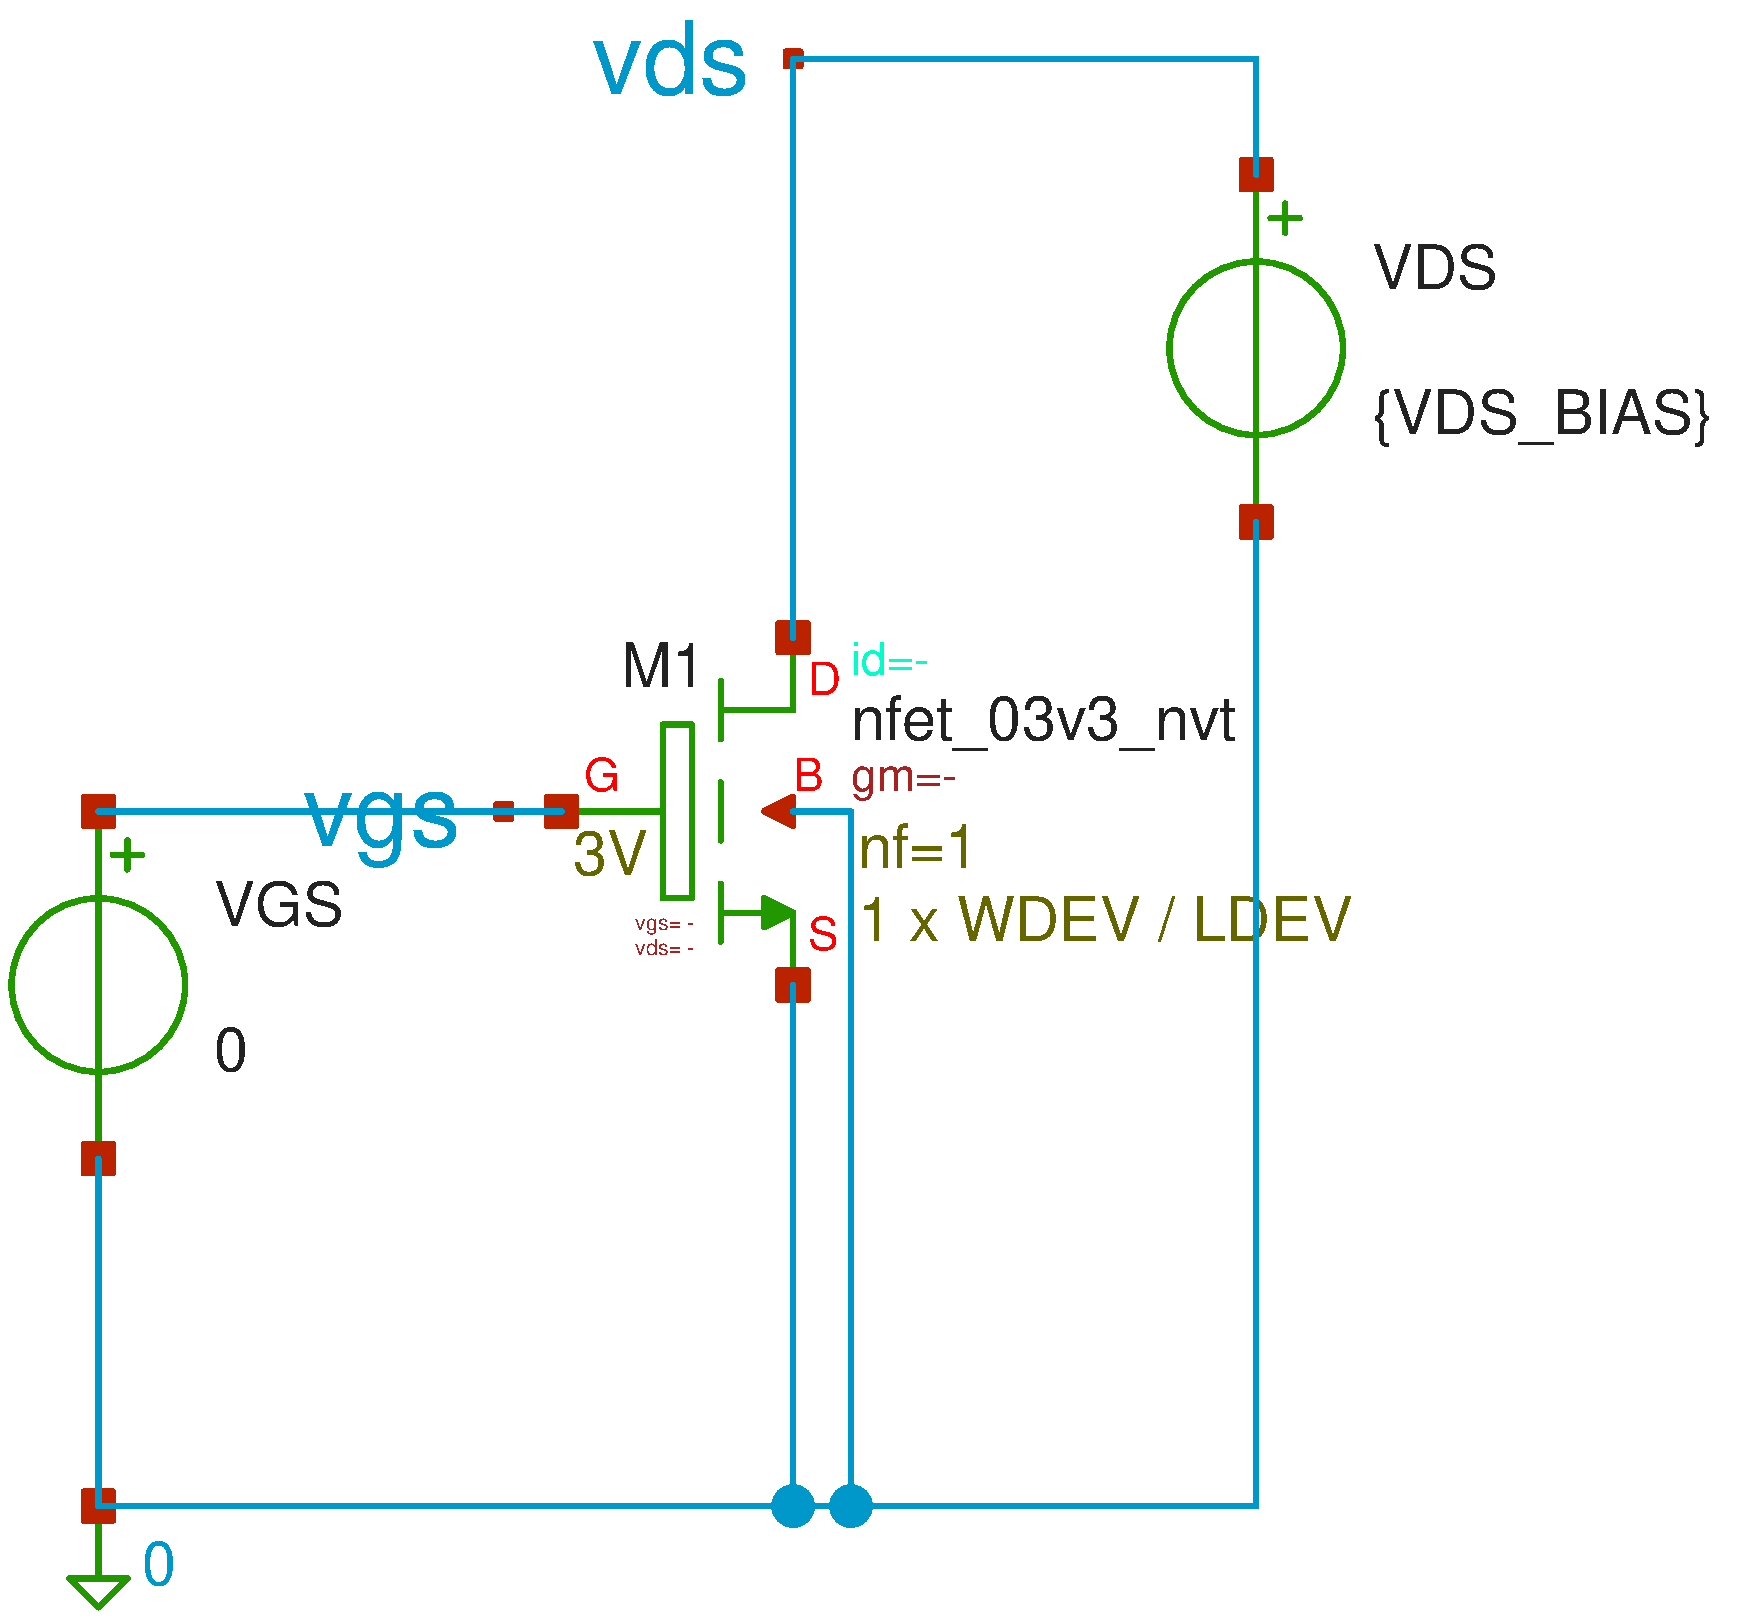
\includegraphics[width=\linewidth]
		{figures/schematics/tb_nfet_03v3_nvt_dc.pdf}
		
		\smallskip
		\small (a) Transfer bench
	\end{minipage}
	\hfill
	\begin{minipage}[t]{0.49\textwidth}
		\centering
		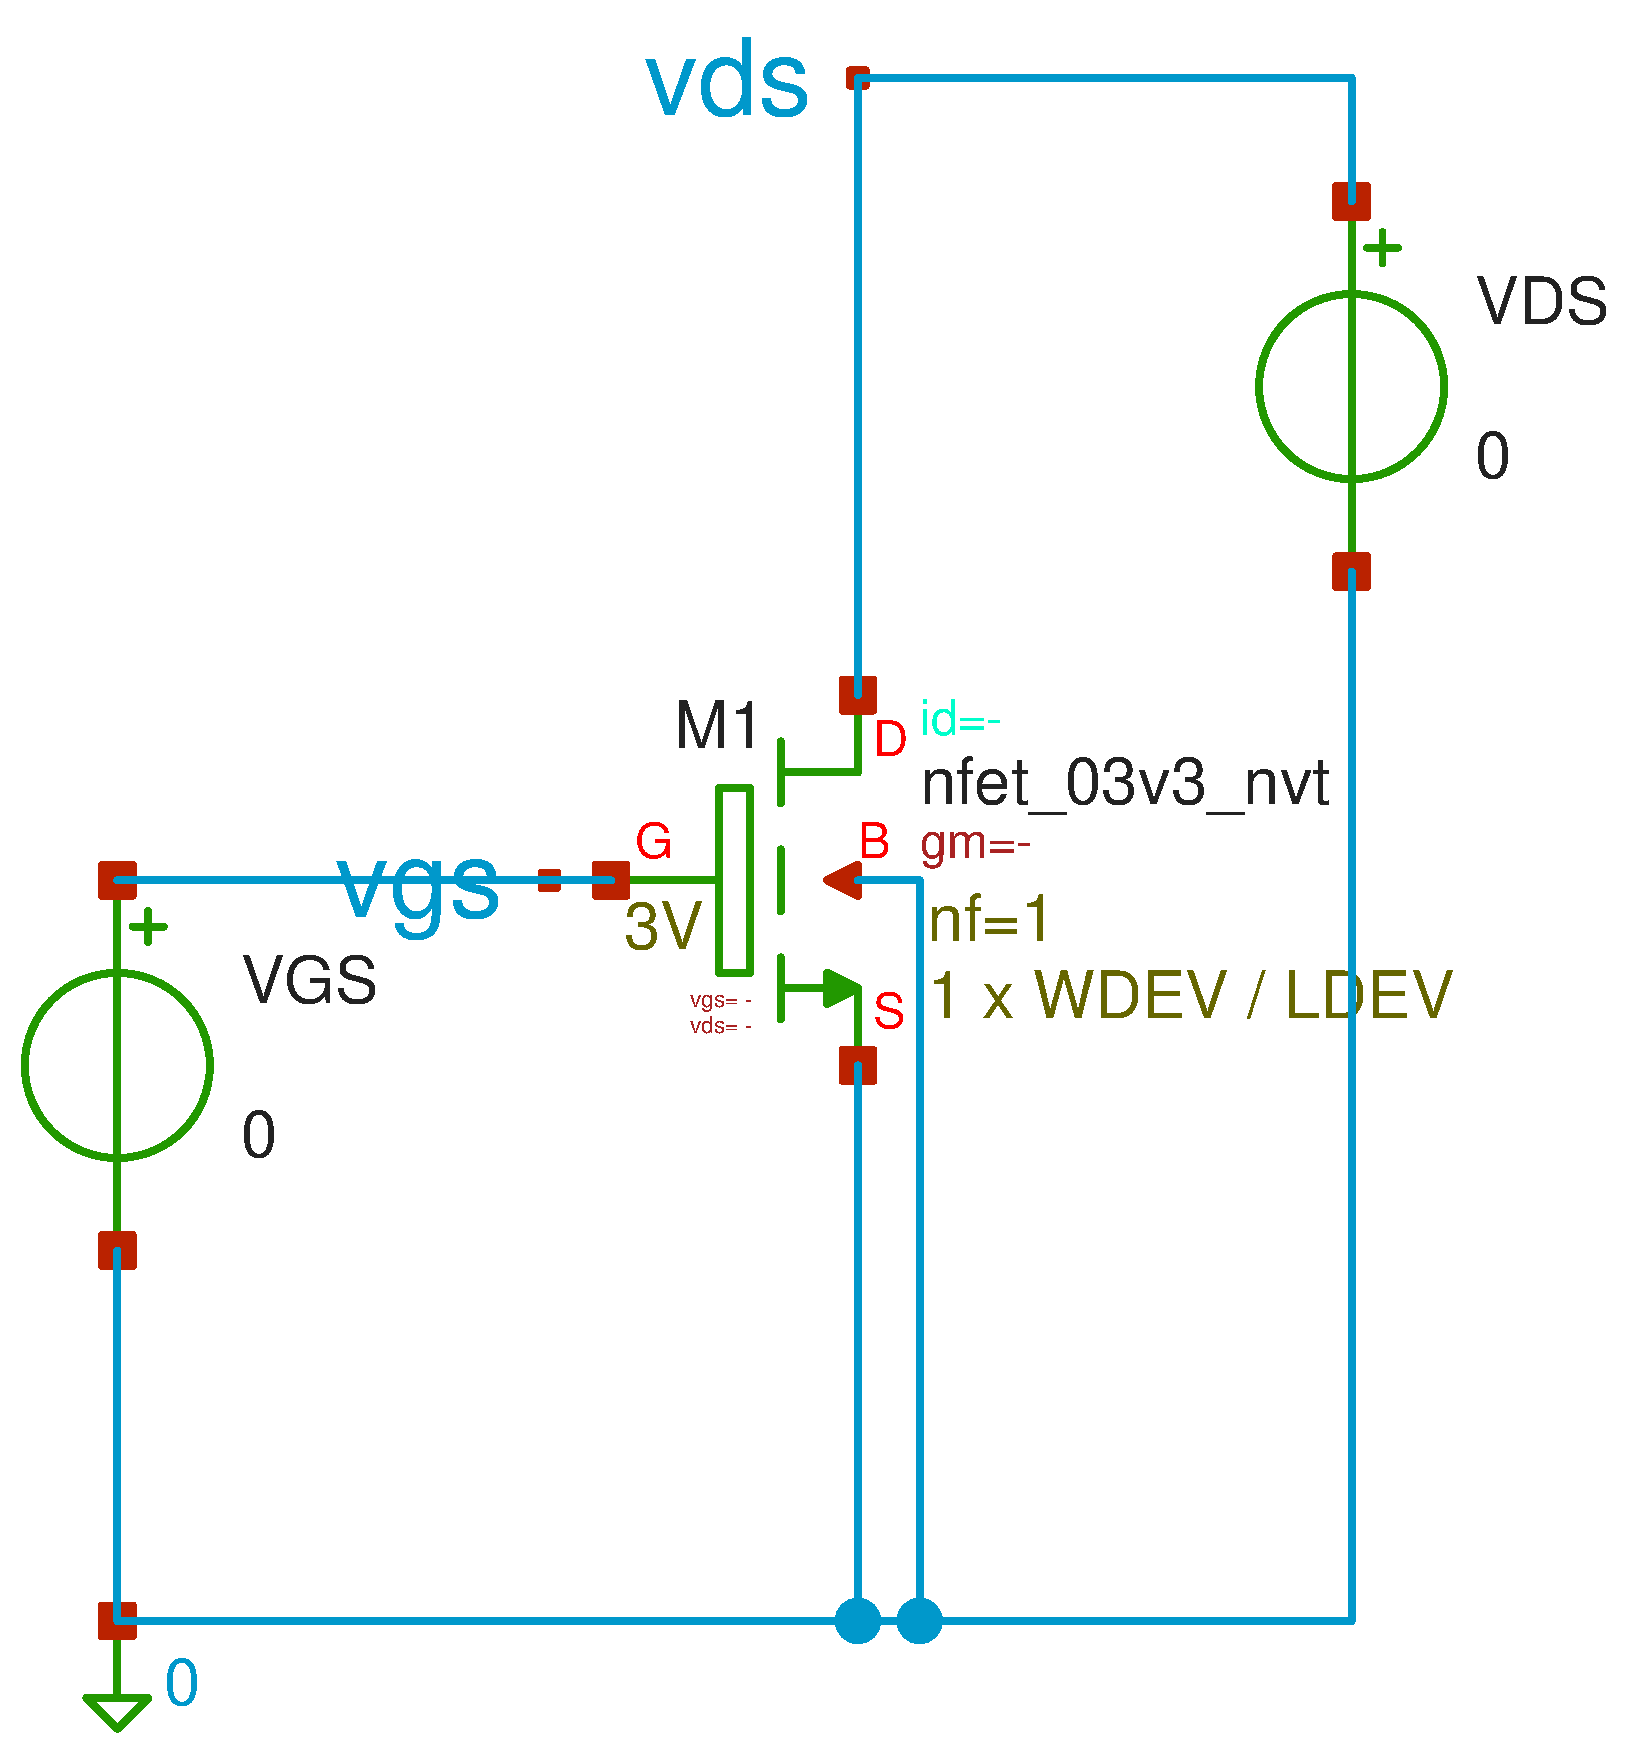
\includegraphics[width=\linewidth]
		{figures/schematics/tb_nfet_03v3_nvt_id_vds.pdf}
		
		\smallskip
		\small (b) Output bench
	\end{minipage}
	
	\caption{Characterization testbenches for the
		\code{nfet\_03v3\_nvt}.}
	\label{fig:tb_nfet_03v3_nvt}
\end{figure}

\begin{figure}[H]
	\centering
	
	\begin{minipage}[t]{0.49\textwidth}
		\centering
		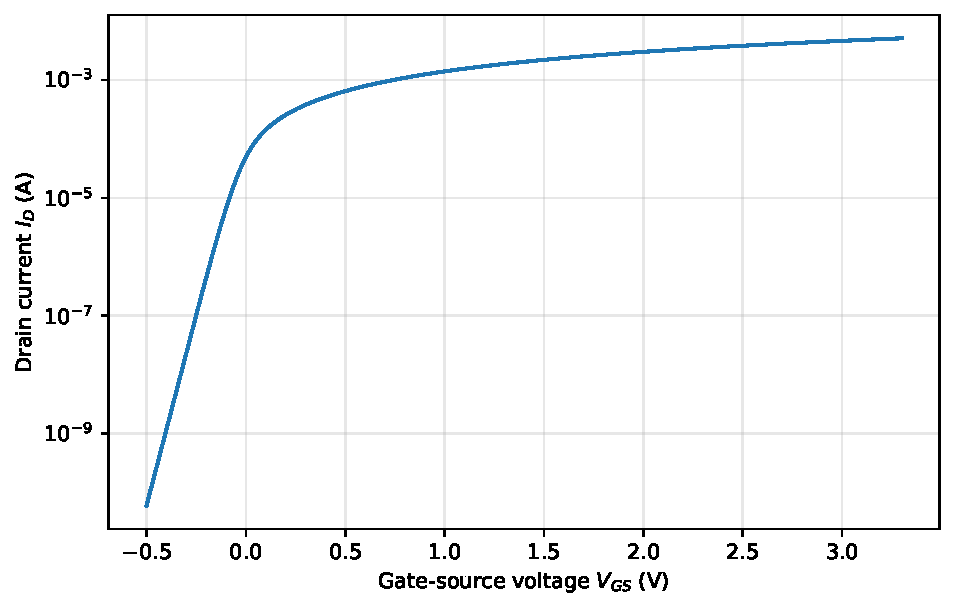
\includegraphics[width=\linewidth]
		{figures/native/nfet_03v3_nvt_id_vs_vgs.pdf}
		
		\smallskip
		\small (a) Transfer characteristic
	\end{minipage}
	\hfill
	\begin{minipage}[t]{0.49\textwidth}
		\centering
		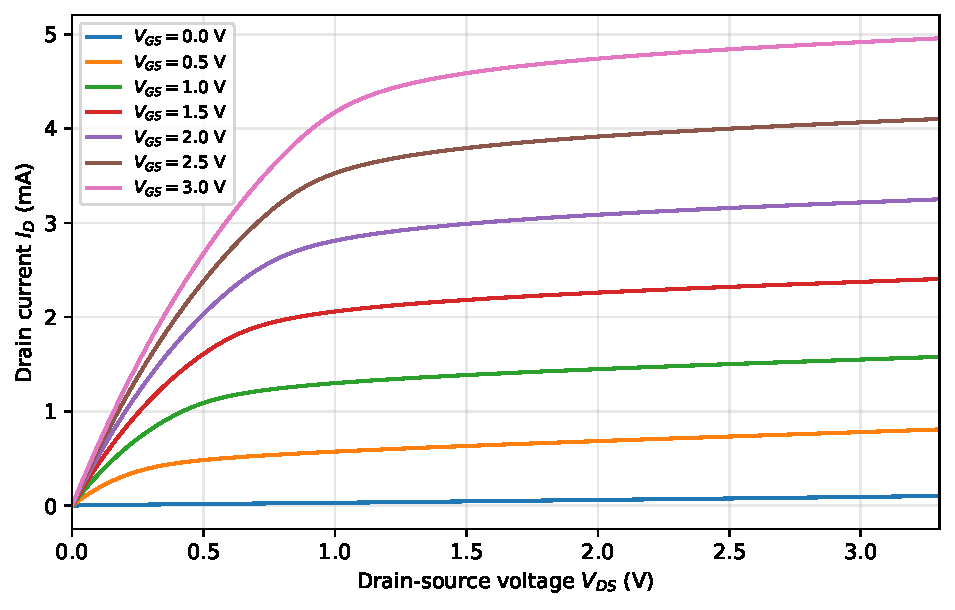
\includegraphics[width=\linewidth]
		{figures/native/nfet_03v3_nvt_id_vs_vds.pdf}
		
		\smallskip
		\small (b) Output characteristics
	\end{minipage}
	
	\caption{Drain-current characteristics of the
		\code{nfet\_03v3\_nvt}.}
	\label{fig:nfet_03v3_nvt_current}
\end{figure}

The device exhibits the expected native behaviour, with an extracted
threshold voltage of approximately
$V_{TH}=\qty{-13.3}{\milli\volt}$ for the reference geometry.
Consequently, measurable drain current is already present at
$V_{GS}=0$.


% ============================================================
% 5-V native
% ============================================================

\subsection{5-V Native NMOS}
\label{sec:nfet_05v0_nvt}

The \code{nfet\_05v0\_nvt} is characterized using

\begin{equation}
	W=\qty{10}{\micro\metre},
	\qquad
	L=\qty{2}{\micro\metre}.
\end{equation}

This geometry is explicitly supported by the available compact-model
bins.

For the reference geometry, the extracted threshold voltage is
approximately $V_{TH}=\qty{52.9}{\milli\volt}$, confirming the
near-zero-threshold behaviour of this device.

The characterization benches are shown in
Figure~\ref{fig:tb_nfet_05v0_nvt}.

\begin{figure}[H]
	\centering
	
	\begin{minipage}[t]{0.4\textwidth}
		\centering
		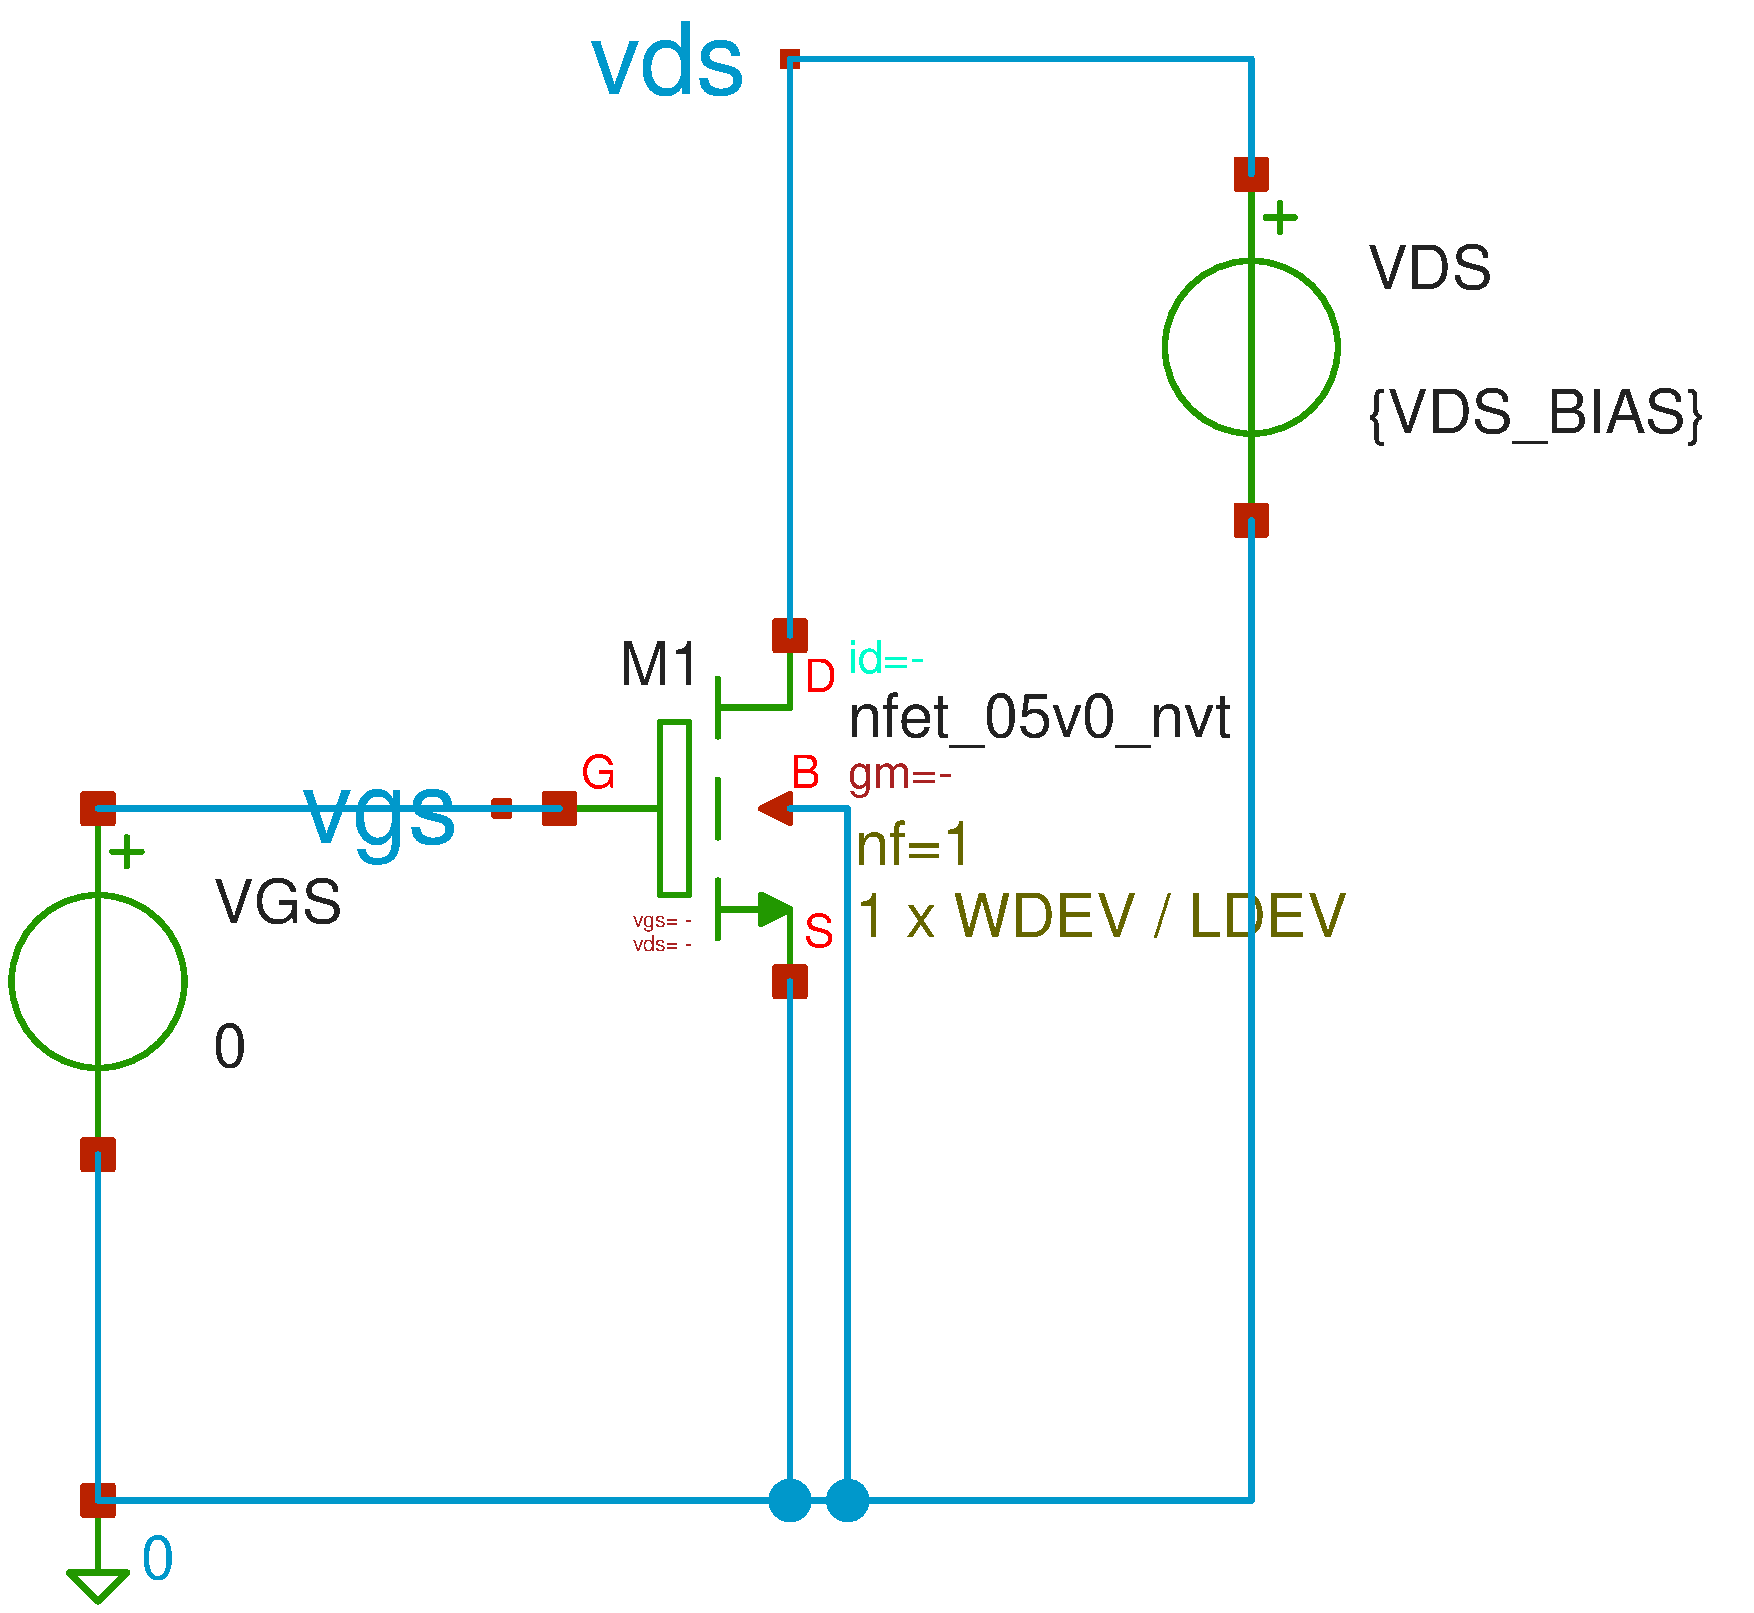
\includegraphics[width=\linewidth]
		{figures/schematics/tb_nfet_05v0_nvt_dc.pdf}
		
		\smallskip
		\small (a) Transfer bench
	\end{minipage}
	\hfill
	\begin{minipage}[t]{0.4\textwidth}
		\centering
		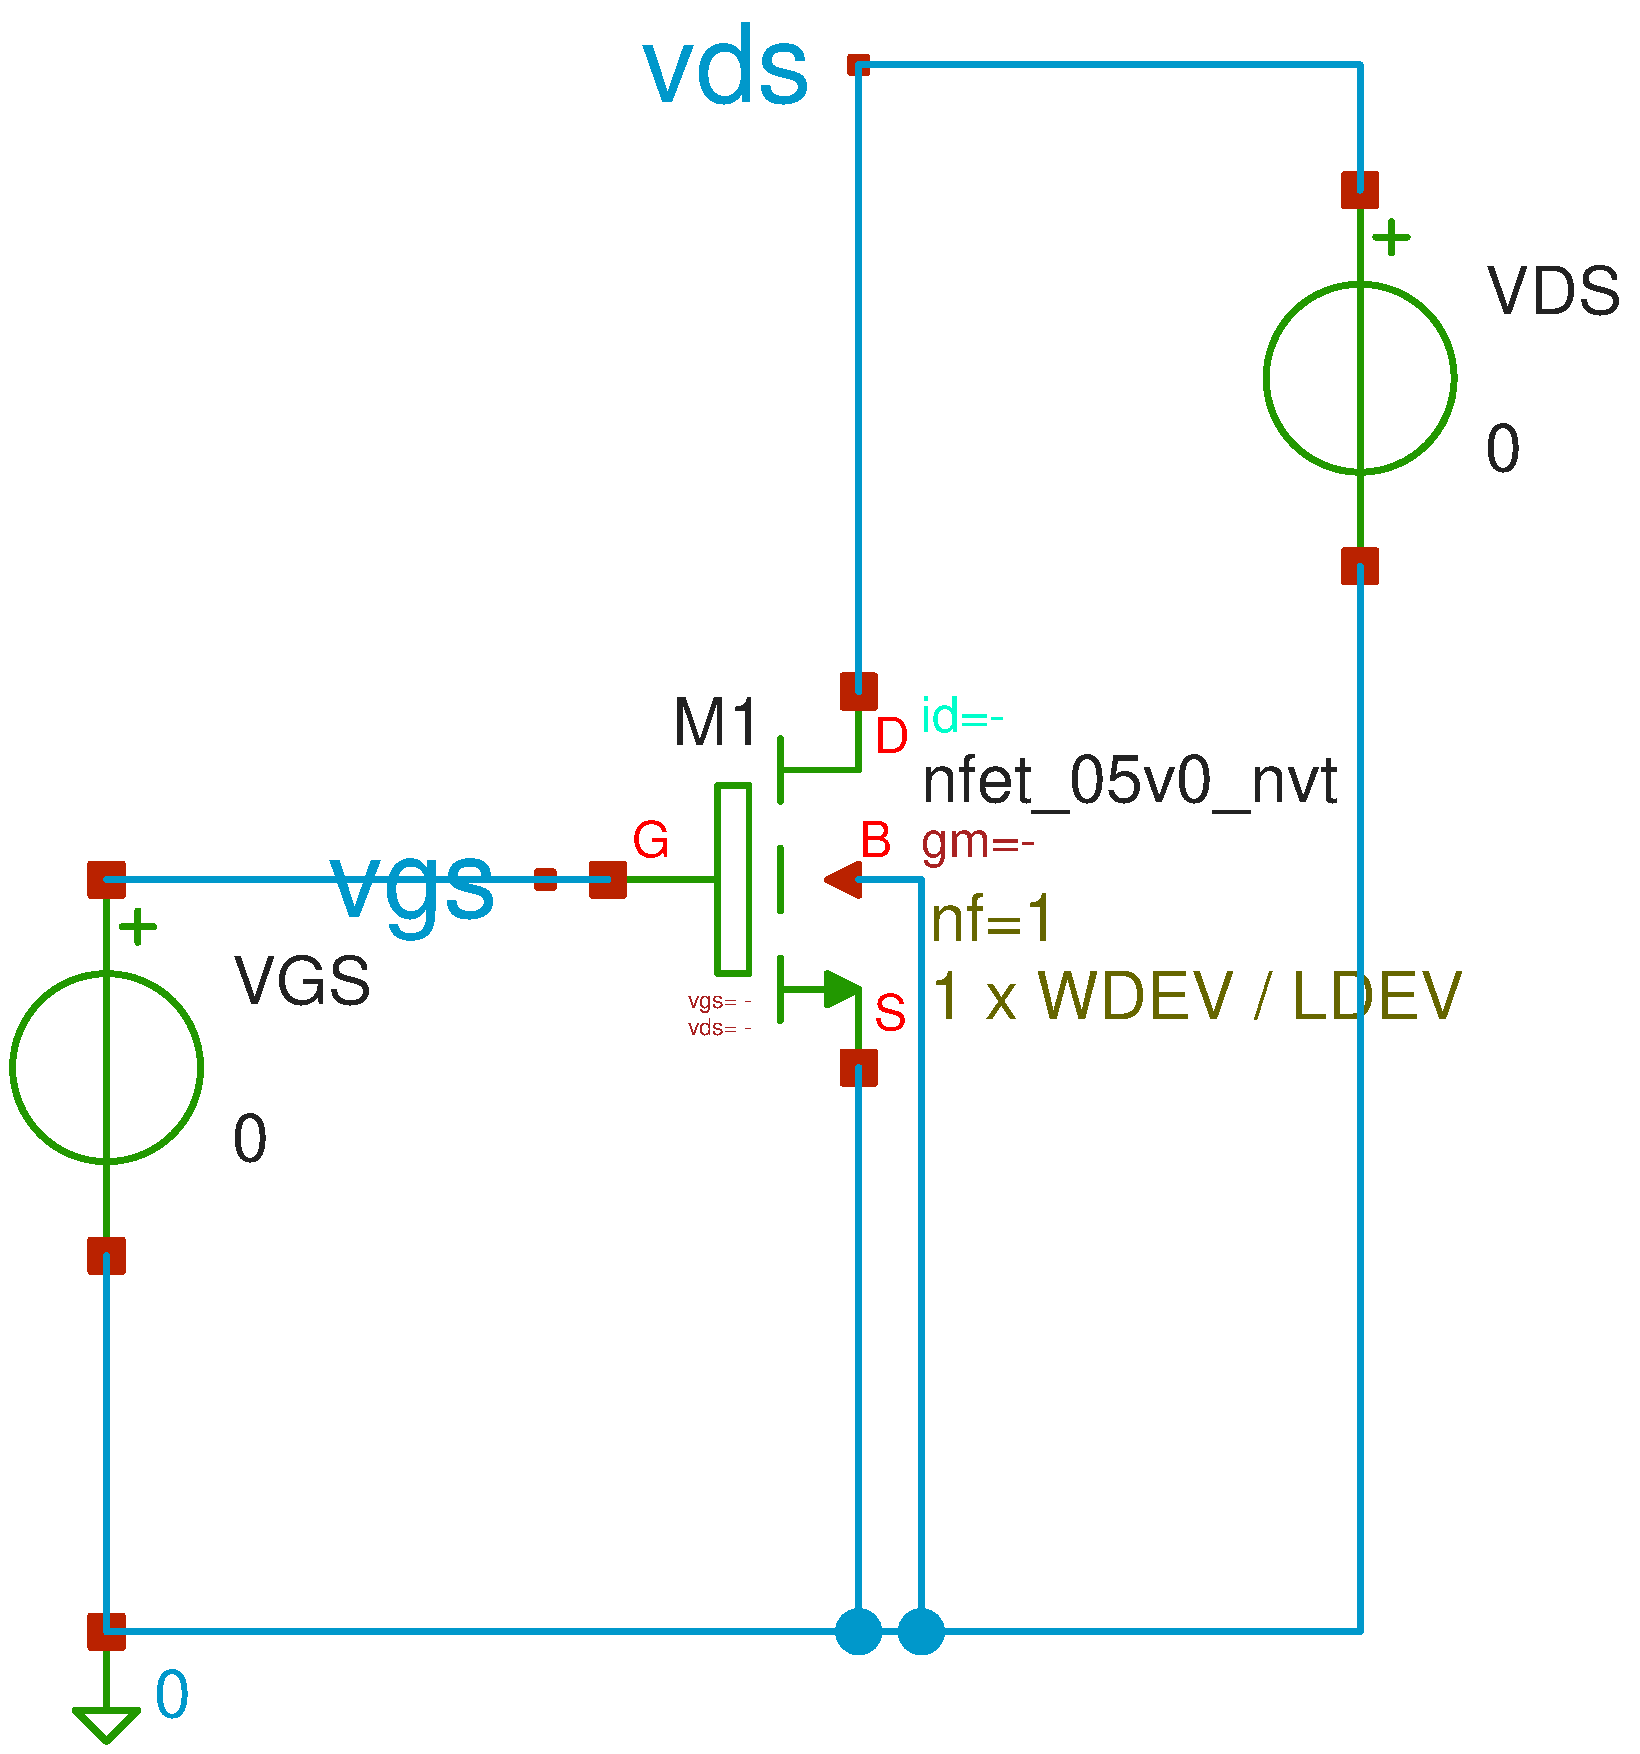
\includegraphics[width=\linewidth]
		{figures/schematics/tb_nfet_05v0_nvt_id_vds.pdf}
		
		\smallskip
		\small (b) Output bench
	\end{minipage}
	
	\caption{Characterization testbenches for the
		\code{nfet\_05v0\_nvt}.}
	\label{fig:tb_nfet_05v0_nvt}
\end{figure}

\begin{figure}[H]
	\centering
	
	\begin{minipage}[t]{0.49\textwidth}
		\centering
		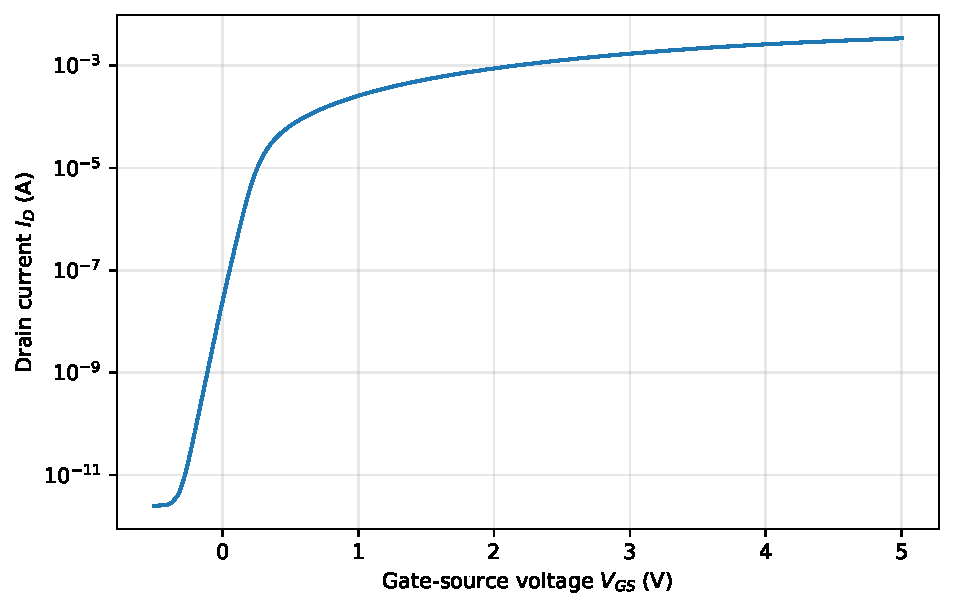
\includegraphics[width=\linewidth]
		{figures/native/nfet_05v0_nvt_id_vs_vgs.pdf}
		
		\smallskip
		\small (a) Transfer characteristic
	\end{minipage}
	\hfill
	\begin{minipage}[t]{0.49\textwidth}
		\centering
		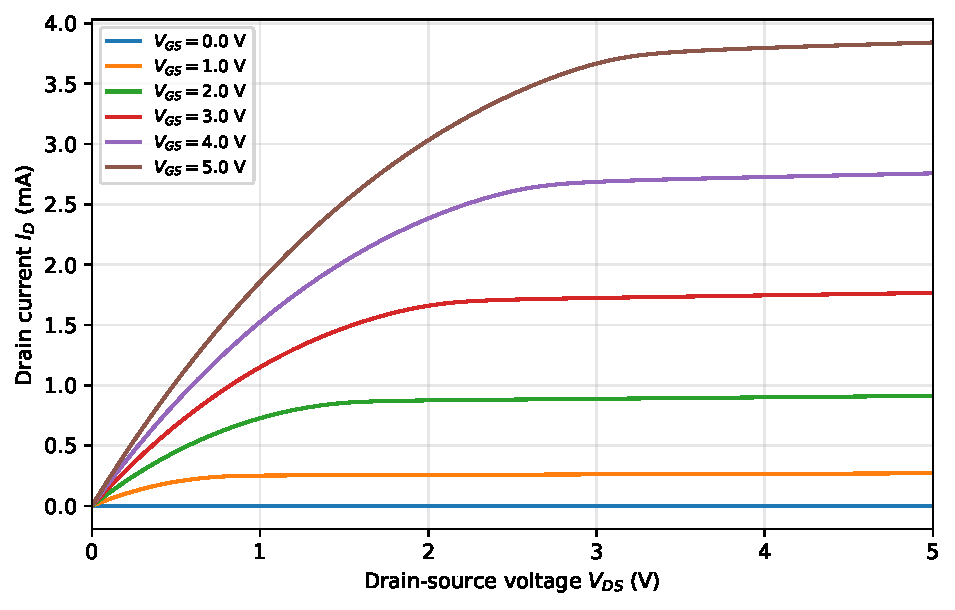
\includegraphics[width=\linewidth]
		{figures/native/nfet_05v0_nvt_id_vs_vds.pdf}
		
		\smallskip
		\small (b) Output characteristics
	\end{minipage}
	
	\caption{Drain-current characteristics of the
		\code{nfet\_05v0\_nvt}.}
	\label{fig:nfet_05v0_nvt_current}
\end{figure}


% ============================================================
% gm/ID comparison
% ============================================================

\subsection{Transconductance Efficiency}

The $g_m/I_D$ characteristics are retained as sizing references for
the two native devices.

\begin{figure}[H]
	\centering
	
	\begin{minipage}[t]{0.49\textwidth}
		\centering
		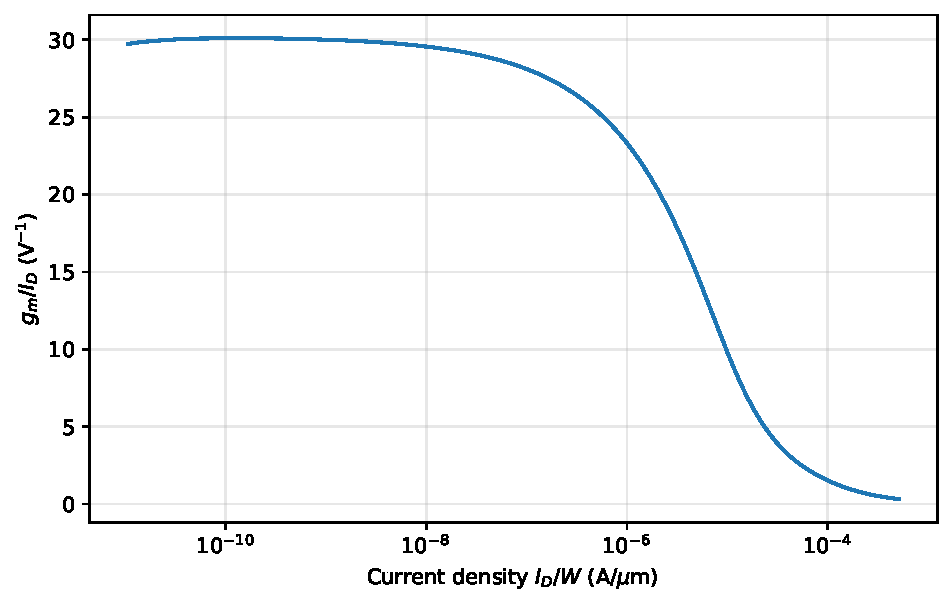
\includegraphics[width=\linewidth]
		{figures/native/nfet_03v3_nvt_gmid.pdf}
		
		\smallskip
		\small (a) \code{nfet\_03v3\_nvt}
	\end{minipage}
	\hfill
	\begin{minipage}[t]{0.49\textwidth}
		\centering
		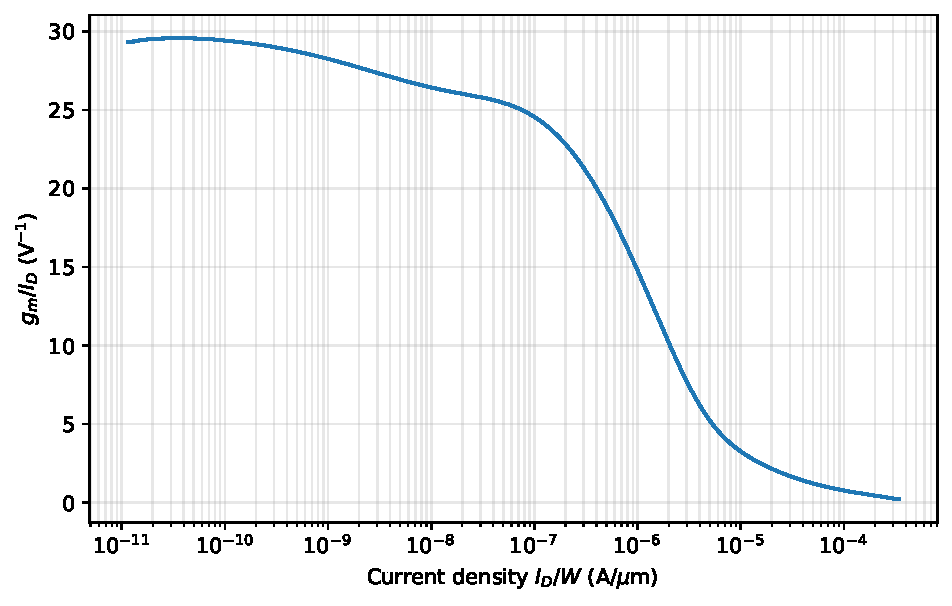
\includegraphics[width=\linewidth]
		{figures/native/nfet_05v0_nvt_gmid.pdf}
		
		\smallskip
		\small (b) \code{nfet\_05v0\_nvt}
	\end{minipage}
	
	\caption{Transconductance efficiency versus drain-current density
		for the characterized native NMOS devices.}
	\label{fig:native_gmid}
\end{figure}


% ============================================================
% Comparison
% ============================================================

\subsection{Native Device Comparison}

Both native devices provide low-threshold operation for circuits where
the standard \qty{1.8}{\volt} NMOS threshold would impose excessive
gate-voltage headroom.

The \code{nfet\_03v3\_nvt} provides the lower-voltage native option,
while the \code{nfet\_05v0\_nvt} extends the usable voltage range but
is available only for a restricted set of compact-model geometries.

The transfer, output, and $g_m/I_D$ characteristics therefore provide
the main information required when selecting between the two devices.